\documentclass{article}

\usepackage{amssymb,amsmath,longtable}

\usepackage[pdftex]{graphicx}
\graphicspath{ {Images/} {Images/eLoss/} }

\usepackage[margin=1in]{geometry}

\usepackage{hyperref}
\hypersetup{
    colorlinks=true,
    linkcolor=blue,
}



\begin{document}

\title{Geane Track Fitting}
\author{Nicholas Kinnaird}
\date{\today}
\maketitle

% \renewcommand{\abstractname}{Assigned Problem}
\begin{abstract}

    In this document I will detail the concepts and mathematics of GEANE track fitting, as well as it's implementation in the gm2 simulation framework. I will also detail the pecularities and intricacies of the code. This is done both for documentation purposes as well as a precursor to sections of my future thesis.

\end{abstract}



\section{Introduction}

  Neccessity for tracking?
  Short intro about hardware? - don't go into electronics

  The Muon g-2 Experiment at Fermilab will use tracking detectors in order to measure positron trajectories for the purpose of determining the beam distribution and characteristics, both for the final result and for general experiment operation. (Sort of a diagnostics tool as well as a secondary detector.) There are 3 tracker stations location at the 0, 12, and 18th sections of the ring, counting clockwise from the top most point of the ring where the inflector resides. Each station consists of 8 tracking modules arranged in a staircase pattern that follows the curvature of the ring. The upstream and downstream trackers reside just after and before vacuum chamber wall respectively. Each tracker module consists of 4 layers of straws with a stereo angle of 7.5 degrees, the first two ``U'' layers oriented with the tops of the straws at a greater radial position, and the second two ``V'' layers oriented with the bottoms of the straws at a greater radial position.

  Link pictures to trackers here for posterity - pictures of trackers in ring, individual module, etc. 

 \subsection{Other physics}

 Physics notes here/elsewhere? 
 Due to the CBO of the beam, 1 tracker accounts for ~90\% of the physics, and a second tracker accounts for much of the remaining. (Find/learn sources for this to explain a bit better..)
 A large percentage of tracks don't hit much of the trackers as the curve in tightly close to the calorimeter.
 ...

\section{In the gm2 Framework}

  \subsection{Branches}

    The GEANE track fitting code is in the main develop branches, except possibly some updates within the feature/trackDevelop branch of gm2tracker. 

  \subsection{fcl Files, Geometry, and Material}

    Event generation before fitting is done using the mdc fcl files in gm2ringsim using the main simulation, where one should also include the tracker dummy plane geometry for truth comparison. At time of writing there are some modified mdc\#-geane fcl files which can readily be used. Only the necessary straw geometry and associated mother volumes, as well as the parallel world dummy planes are necessary to fit tracks, though including other geometry will of course change particle behaviour. All 3 main trackers are included in their original positions. There is a fcl parameter useSD to turn on and off the straw sensitive detectors so that in the reconstruction phase hits are not regenerated.

    Reconstruction is performed using RunGeane.fcl in gm2tracker on the output from the above. Parameter useSD for the straws should be turned off. The fcl file loads all 3 trackers necessary for symbol and name definitions, but such that tracker 0 is rotated such that the tracking planes are parallel to the global geant X axis (using the rotateArcTracker fcl parameter for the ArcService). This is done to avoid the issue of error propagation instability close to the Z axis, as detailed in \href{http://gm2-docdb.fnal.gov:8080/cgi-bin/ShowDocument?docid=4567}{DocDB 4567} while at the same time still observing the correct azimuthally symmetric 2D field for the tracks. Track hits are rotated from their separate trackers to this one tracker frame with the geaneWorld0, geaneWorld12, and geaneWorld18 transforms defined at the bottom of StrawTrackerService.cc (or the cadmesh version). In the future, if fields or geometries are not identical between trackers, the details here will have to be improved.

    Fcl parameters exist for the StrawTrackerService and StrawsService in order to turn material on or off at will, ``materialTracker'' and ``material'' respectively. The rest of the geometry has to be manually changed and rebuilt in order to remove material. These include VacuumChamberCadMesh and the World, as well as the ``buildSupportPost'' option in strawtracker.fcl and strawtracker\_standAlone-staggered.fcl, ``buildTrolly'' in vac.fcl (where the associated material is hardcoded in), and ``trolleySupportMaterial'' also in vac.fcl. Make sure to have the same material settings for the reconstruction as how the events were generated.. This is purely for debugging the tracking.

    The reconstruction code links to geaneFitParams.fcl in gm2tracker which has many variables for changing momentum spreads, straw measurement errors, random seeds, toggling truth info, etc. Things get more complicated here so ask me before trying to play with this stuff.

  \subsection{GEANE TrackFitting}

    The GEANE track fitting routines consists of a couple of main files within gm2tracker. Track candidates from upstream in the reconstruction chain are the input to this code. A single GEANEArtRecord is produced for each event or track, and is passed from one method to another, constantly being updated as the track fitting iterates along. See below for a quick summary of the method flow, and a table for the data objects within GEANEArtRecord. 

    \begin{enumerate}

      \item{\bf{GeaneReco\_module.cc}} \\
      This file consists of the main code which sets up the GEANE track fitting, pulls in upstream data products, interfaces with both Geant4 and the gm2 art framework, and outputs TrackStateArtRecords and TrackArtRecords for use downstream. It's methods consists of:

        \begin{itemize}

          \item{produce} \\
          General overriden produce method. Calls main track fitting code on an event by event basis. Produces data products for downstream use.

          \item{InitializeGEANE} \\
          Geant4 GEANE initialization method called by the constructor, once per run.

          \item{trackFitting} \\ 
          Sets up variables and objects for track fitting after reading in upstream data products (track candidates and dummy planes). Contains main track fitting iteration loops. Also contains complex L/R sequence checking routines which can be ignored for now (and probably need to be changed at some point).

          \item{modifyMeasuredParams} \\ 
          Short method for L/R sequence checking stuff, can be ignored for now. Just modifies measured parameters based on particular sequence

          \item{errorPropagation} \\ 
          This method tracks particles through the detector using Geant4 error propagation routines with the correct geometry and field. It builds transport matrices, error matrices, and predicted parameters which are the objects used for fitting the track. It tracks on a plane by plane and step by step basis. These routines can be used to track particles forwards and backwards, where the forwards tracking is used in the code. Changing to backwards tracking would be very non-trivial. Add more detail here later..

          \item{angleCorrection} \\
          Method to iteratively correct measured parameters from a radial DCA value to a U or V value based on the momentum of the track and approximating a constant field within the straw. Also corrects the errors using a simple straight line approximation which is good enough.

        \end{itemize}

      \item{\bf{GeaneFitter.cc}} \\
      This file consists of the main track fitting chi2 algorithm. It multiplies measured parameters, predicted parameters, error matrices, and transport matrices together to produce a chi2 for the track and an improvement to the starting paramters. It also reads in the measured hits errors in order to properly fit the track. There is a fcl parameter matrixDebug which can be used to turn on or off the many large matrix cout debugging statements.

        \begin{itemize}

          \item{TrackCorrelation} \\
          The main matrix multiplication routines.

          \item{preSequenceChecking} \\
          A method in order to create a hybrid wire / U or V error matrix for L/R sequence checking. Only called once per event.

          \item{sequenceChecking} \\ 
          The main L/R sequence checking method for an individual event. This method is called many thousands of times as each U or V sequence is checked. Ignore for now.

          \item{convertTo} \\
          Some methods for converting Eigen 5 vectors from GeV cm to MeV mm and vice versa.

        \end{itemize}

      \item{\bf{GeanePlots\_module.cc}} \\
      The main analyzer/plotting module which runs on the output GEANEArtRecords produced upstream. This creates many plots including chi2 distributions, p value distributions, number of iterations, track parameter, residuals, pulls, etc. Truth information for these plots is currently necessary as written, but can be take out in the future for real data. There are some fcl paramters to make cuts on different parameters. There are also some other plotter modules which are similar but much reduced in scope.

      \item{\bf{GEANESingleEventViewer\_module.cc}} \\

      \item{\bf{GeaneFailedPlots\_module.cc}} \\

      \item{\bf{GeanePoorEvent\_module.cc}} \\

      \item{\bf{refit geane stuff?}} \\

    \end{enumerate}


    Quick summary of the track reconstruction method flow: The main file StrawTrackLeftRightGEANE\_module is called and sets up both the Geant4 world and the GEANE routines. Produce is called per event, a GEANEArtRecord is created, and upstream track candidates are pulled in and the relevant parameters are converted to necessary track fitting objects within the method trackFitting. The methods errorPropagation, angleCorrection, and TrackCorrelation (in GEANEFitter) are called iteratively within a loop until track fitting succeeds or fails. The relevant parameters of the updated GEANEArtRecord are then converted to TrackArtRecords and TrackStateArtRecords for downstream use, and the analyzer/plotter modules are called for output checking.

    Note: Ignore copious LR ambiguity solving code for now. When last checked it was working pretty well but not perfectly, and it needs to be studied more. Many changes have been made to other code which will probably break the interfaces to the LR code as well. Also all of this LR stuff might be pulled out and placed into other tracking code modules before and after the GEANE code, but that is unclear.


\begin{longtable}{|p{16cm}|}
% \scriptsize
\caption{GeaneArtRecord.hh active variables. This is subject to change. GeaneArtRecord contains vectors of variables on planes, as well as larger objects containing information about the whole track. improve comments here and in the code - don't forget to update this if/when I change things in the code} 
% \begin{tabular}{|p{16cm}|}

  \\ \hline
% Variable \\
%   \hline

art::Ptr \textless{} gm2strawtracker::TrackCandidateArtRecord \textgreater{} candidate \\
\textit{One track corresponding to one candidate corresponding to one GEANEArtRecord for the whole track.} \\ \hline

std::vector\textless{} art::Ptr\textless{} gm2truth::GhostDetectorArtRecord \textgreater{} \textgreater{} dummyPlaneHits \\
\textit{Associated dummy plane hits on planes aligned with straw wires, vector consists of hit dummy planes corresponding to hit wire planes (if a straw plane was skipped but that dummy plane was hit, it is not included in this vector. Vector has size N = num hits in straws that form the track.)} \\ \hline

int failureMode \\ 
\textit{Different failure modes for failed track reconstruction, 0 means it passed.} \\ \hline

double chi2 \\ 
\textit{Chi2 for whole track.} \\ \hline

std::vector\textless{}double\textgreater{} chi2Iterations \\
\textit{Chi2s for whole track for different iterations.} \\ \hline

std::vector\textless{}double\textgreater{} chi2Planes \\
\textit{Individual chi2s on each plane which add up to total chi2, vector consists of hit planes with size N.} \\ \hline

int numIterations \\
\textit{Number of iterations to converge.} \\ \hline

unsigned int dof \\
\textit{DoF of track = number of hit planes - 5 track parameters.} \\ \hline

double chi2DoF \\
\textit{chi2/dof} \\ \hline

double pValue \\
\textit{Fit pValue for whole track.} \\ \hline

double energyDiff \\
\textit{energy loss between first and last hit in track - from truth, for material characterizing} \\ \hline

std::vector\textless{}G4double\textgreater{} startingTrackParameters \\
\textit{Starting parameters for track: size 6, 3 position then 3 momentum, x y z px py pz, best starting parameters updated after each iteration, starting parameters x position defined before first hit.} \\ \hline

std::vector\textless{}G4double\textgreater{} startingTrackGuessOffsets \\
\textit{Size 10, x y z px py pz p 1/p pu/px pv/px offsets in different starting track parameters for plotting purposes.} \\ \hline

int trackNumPlanesHit \\ 
\textit{Total number of planes hit.} \\ \hline

int trackFirstPlaneHit \\ \hline

int trackLastPlaneHit \\ \hline

std::vector\textless{}int\textgreater{} trackPlanesHitList \\
\textit{List of hit planes, with missed planes excluded from the vector. Ex. 1 2 4 5 8 9} \\ \hline

\textit{Sequence information excluded from this table for now.} \\ \hline
        % int trueUSequencePosition; ignore sequence information for now
        % int pseudomeasuredUSequencePosition; ignore sequence information for now
        % int trueVSequencePosition; ignore sequence information for now
        % int pseudomeasuredVSequencePosition; ignore sequence information for now
        % int trueFullSequencePosition; ignore sequence information for now
        % int pseudoMeasuredFullSequencePosition; ignore sequence information for now
        % double trueChi2Difference;
        % double pseudoMeasuredChi2Difference;

std::vector\textless{}std::vector\textless{}G4double\textgreater{} \textgreater{} wireUVPositions \\
\textit{Wire center U and V postions, first vector is track param vector size 5 (0 1 2 unfilled, 3 is U, 4 is V), second vector is planenumber from 0 - 32  (formatted this way to align with other similar vectors - can probably be reduced.)} \\ \hline

std::vector\textless{}G4double\textgreater{} measuredDCAs \\
\textit{Vector of measured DCAs for hit planes, with size 33. Mainly to hold on to smearing values for now.} \\ \hline

std::vector\textless{}G4double\textgreater{} UVerrors \\
\textit{Vector of UV measurement errors for planes 0-32. Built in order to accomadate varying errors in the future.} \\ \hline

std::vector\textless{}G4double\textgreater{} planeXPositions \\
\textit{Vector of X postions of hit wire planes with size 33 (0 - 32), 0 plane being in front of the first module that was hit.} \\ \hline

std::vector\textless{}std::vector\textless{}G4double\textgreater{} \textgreater{} geaneMeasuredParameters \\
\textit{Measured GEANE parameters, first vector is param num 0 - 4, second vector is plane number 0 - 32, units are MeV mm. 1/P, Pu/Pz, Pv/Pz, U, V - only U or V is filled at the start of the GEANE fitting module.} \\ \hline

std::vector\textless{}std::vector\textless{}G4double\textgreater{} \textgreater{} geanePredictedParameters \\ 
\textit{Predicted GEANE parameters, first vector is param num 0 - 4, second vector is plane number 0 - 32, units are MeV mm. 1/P, Py/Px, Pz/Px, Y, Z - all params filled in tracing stage of GEANE fitting module - coord system has to be orthogonal - converted to UV locally in the fitting module.} \\ \hline

std::vector\textless{}Eigen::MatrixXd\textgreater{} geaneTransportMatrices \\
\textit{Units of GeV cm - transport matrices between planes tracked to in GEANE fitting module, 5x5 objects. Vector has size 33.} \\ \hline

std::vector\textless{}Eigen::MatrixXd\textgreater{} geaneErrorMatrices \\ 
\textit{Error matrices on tracked to planes, units GeV cm, size 33.} \\ \hline

std::vector\textless{}Eigen::VectorXd\textgreater{} extendedParamPredictedInUVEigen \\ 
\textit{Predicted parameters in UV space as an eigen object (converted from geanePredictedParameters above) for calculation convenience and some LR information storage. Order of vectors is switched here, first is planenum, second is paramnum, units are MeV mm.} \\ \hline

\textit{Objects below here are full track objects with larger sizes, mostly held on to for fast sequence checking, with some used in other parts of the code. Units GeV cm.} \\ \hline

std::vector\textless{}Eigen::MatrixXd\textgreater{} extendedTransportMatrixBegToEnd \\
\textit{Accumulated/combined transport matrices from starting plane to all following planes.} \\ \hline

Eigen::MatrixXd extendedCombinedTransportMatricesTranspose \\
\textit{Transpose of larger eigen object composed of above begtoend transport matrices.} \\ \hline

Eigen::MatrixXd extendedCovarianceTotal \\
\textit{5x5 total covariance matrix for track, except \textbf{INVERTED}.} \\ \hline

Eigen::MatrixXd extendedReducedMatrix \\ 
\textit{Total error correlation matrix, reduced to size NxN (N = num planes hit).} \\ \hline

Eigen::MatrixXd extendedReducedMatrixInverseLargeErrors \\ 
\textit{Inverse of above but with larger errors from initial wire fitting, for LR checking.} \\ \hline

Eigen::MatrixXd extendedModifiedReducedMatrix \\ 
\textit{Reduced matrix from above that's going to be modified into a hybrid error matrix separately for U and V fits but that needs to be held onto for all sequences.} \\ \hline

  \hline

% \end{tabular}
\end{longtable}

\subsection{Code details}

Building and multipilying transport and SC2SD matrices
Modifying measured parameters based on momentum angle/field and previous predicted
Converting things to eigen objects

JacobianToUV stuff - or combine with other coordinate transform stuff
Matrix accumulation/reduction
Notes on loop indices, start points and such

\subsection{Code peculiarities / notes}

Where to structure this in the file?

Notes on coordinate systems I use - UV pointing outward vs XYZ, XUV x being forward, UVW in geante src, maybe IJK/TUV in one paper-prob not, GeaneTrackerWorld[0,12,18], rotateArcTracker (bit more specific), magnetic field access coordinates?, JacobianToUV

accessing the field in a specific way



\section{gm2Geane package in artg4 - eloss, brems, ionizations, msc}

See many docdbs by Nick Kinnaird on geane updates for more info if wanted. Summary of stuff here.


There is a folder under artg4/gm2Geane, where slightly (but importantly) modified geant/geane code that the geane track fitting uses is located. Most importantly is that the reconstruction was taking too much energy away from the particle during propagation due to bremsstrahlung, so that has been removed. (Thanks James for help with this.) (Probably explain flow of file - extrapolator tables etc.).

Besides those associated files, all files from the geant folder ``error\_propagation'' have been copied into this directory as well, with the only non-name changes lying in gm2GeaneFreeTrajState.cc. (Many files had to be copied due to naming/linking - some could probably have been omitted but I decided to copy the whole folder.) Ionization and multiple scattering errors have been modified according to Lavezzi thesis (explain more) - with no improvement in results unfortunately. (Probably turn defaults back to original code (still gm2Geane) with the option to turn things on somehow if desired - at least leave them in for future tuning.)

Should I go more in depth about the error\_propagation/gm2Geane source code? Probably - at least for certain main files.


Add many plots and pictures of things - pulls, single events, tracks, etc etc.

\begin{figure}[h]
\caption{caption - landau tail, from ionizations, brems, blah blah}
\centering
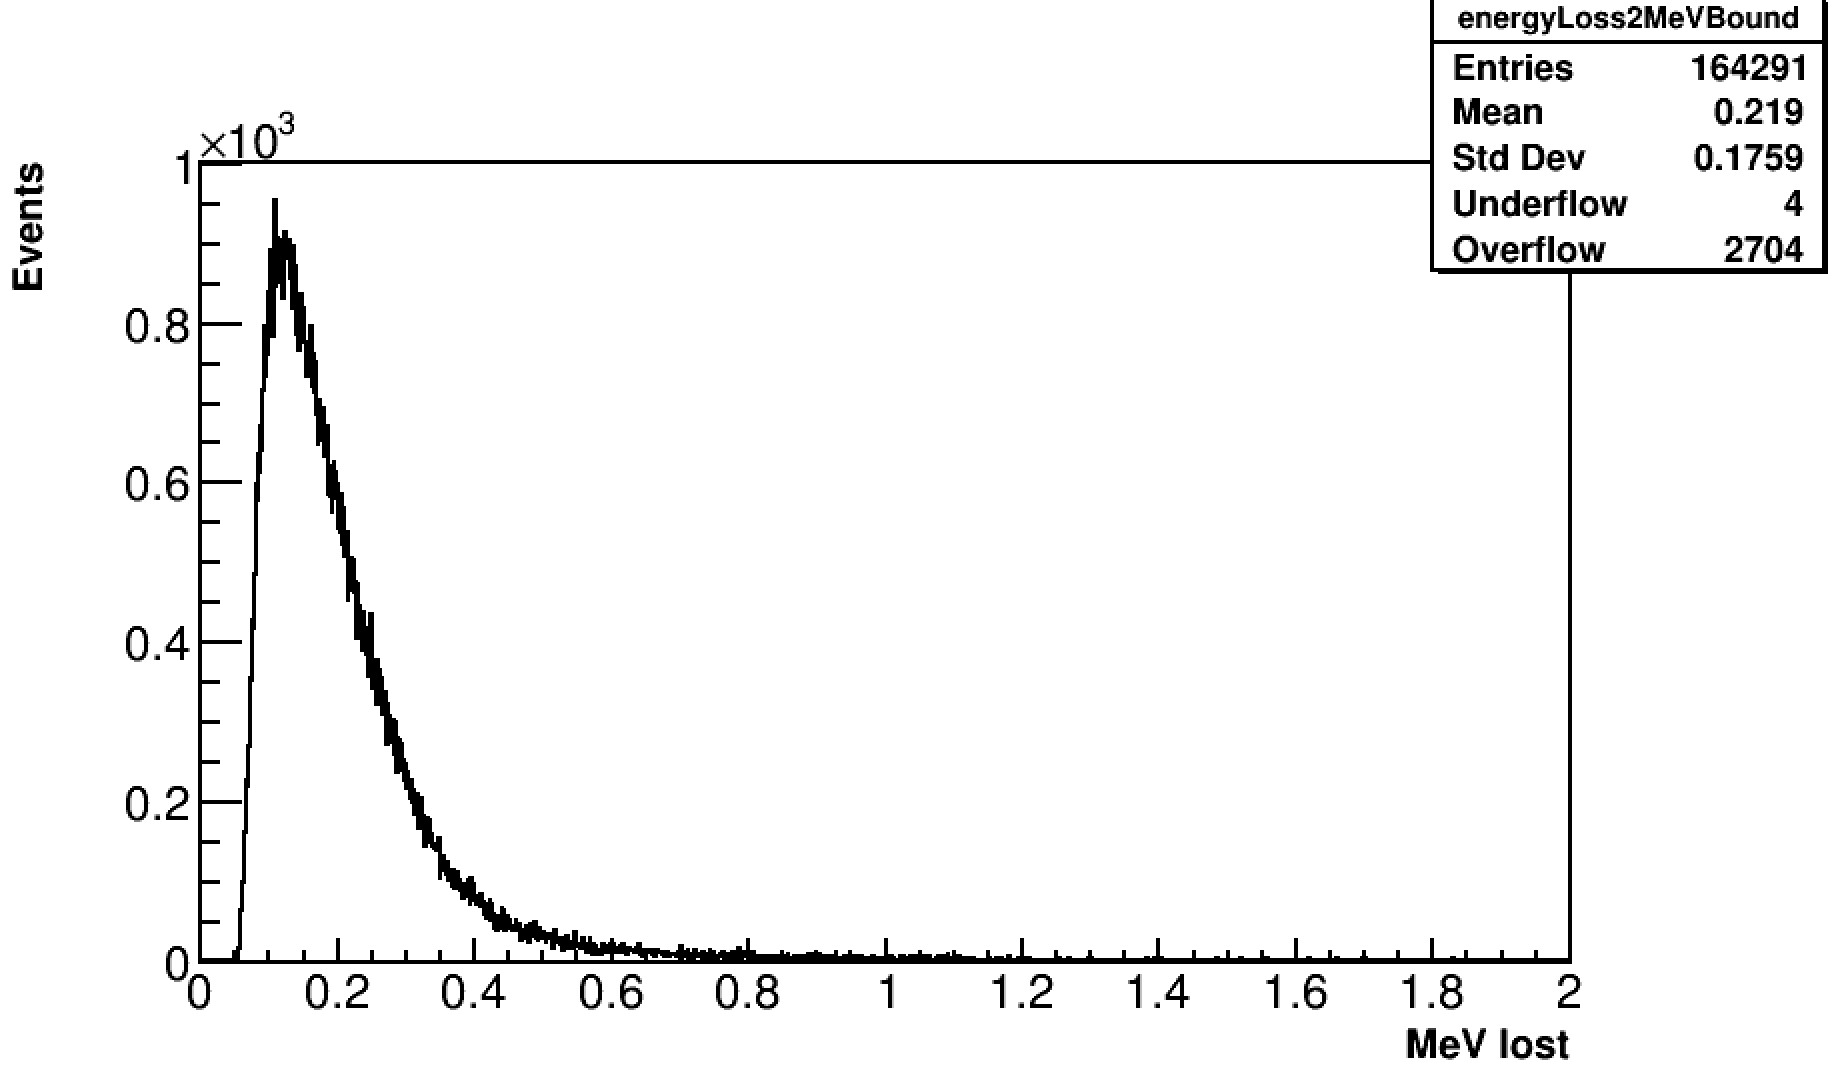
\includegraphics[width=1.0\textwidth]{eLoss}
\end{figure}

\begin{figure}[h]
\caption{caption - brems were adding too much energy back in - fixed event, blah blah, notice scale change}
\centering
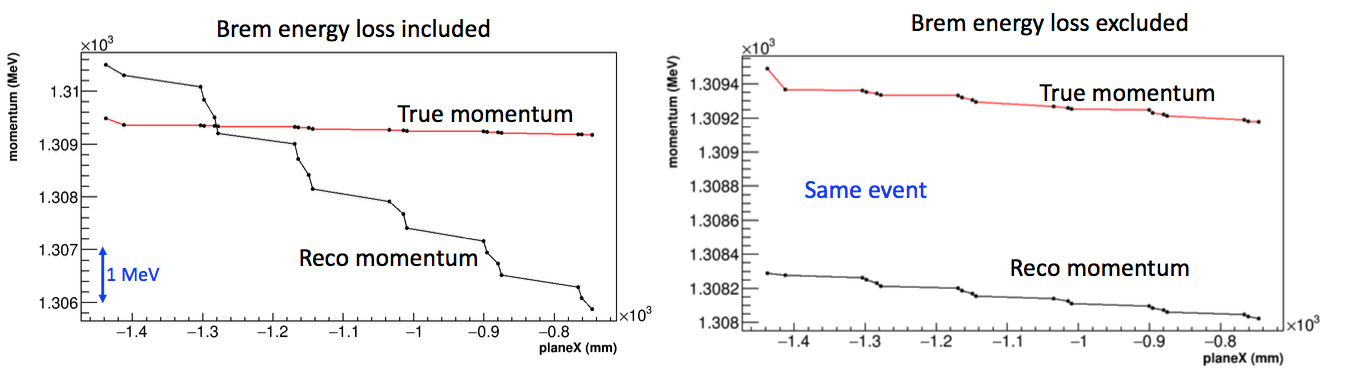
\includegraphics[width=1.0\textwidth]{bremComparison}
\end{figure}


\section{notes and other}

  starting error matrix

  linking equations to code variables

  initial errors into tracing/error propagation?


\section{Formalism - Appendix? }

% $$ on both sides to separate into single line equations, $ on each side for in-text

The purpose of this section is to give a full account of the GEANE formalism used in the tracking code in one place, in a way that makes the most sense to me, as well as it's unique adaptations. For the original source of this material see first the GEANE manual (cite here) and then the Innocente paper (cite), Strandlie paper (cite), and Lavezzi thesis GEANE section (cite). 

It is also important to note that there is a sort of linquistic defficiency in that GEANE refers to both the error propagation code (Geant4 source routines), as well as the general $\chi^{2}$ minimization algorithm, depending on the reference. Locally, I will try and distinguish clearly between the two.


\subsection{Coordinate Systems}

The only material not covered here in full detail is the mathematical explanation of reference frames, for which one should see the reference papers. It suffices to summarize as follows: GEANE objects (matrices and parameter vectors) are defined and calculated in the Geant4 source code in the free particle system as always. Then there is an intermediate surface system defined in XYZ, as the Geant4 surface trajectory system must be defined in an orthogonal coordinate system, before which parameter objects are converted to the most natural detector system of XUV. (Important note - be very careful with coordinate system variables, letters are reused between different papers and code bases with different configurations and meanings constantly.)

$1/p, \lambda, \phi, y_{\perp}, z_{\perp}$, free system

$1/p, py/px, pz/px, y, z$, surface system

$
\begin{pmatrix}
u \\
v \\
\end{pmatrix} =
\begin{pmatrix}
-\sin{\theta} & -\cos{\theta} \\
\sin{\theta} & -\cos{\theta}\\
\end{pmatrix}
\begin{pmatrix}
y \\
z \\
\end{pmatrix}
$, yz to uv matrix, the 5x5 transformation is just a 1 in the top left corner, and then this matrix in the remaining 2 diagonal blocks

$1/p, pu/px, pv/px, u, v$, uv system


\subsection{Matrix Stuff}


$\chi^2 = \sum_{i=1}^{N} [(p_{i}(p_{0})-x_{i})^{T}(\sigma_{i})^{-1}(p_{i}(p_{0})-x_{i})]$, $p_{i}$ the average predicted from some starting $p_{0}$, only diagonals of $\sigma_{i}$ non-zero, measurement error plus material error

$\sum_{i=1}^{N} T^{T}_{i0}(\sigma_{i})^{-1}(p_{i}(p_{0})-x_{i}) = 0$

$p_{0}' = p_{0} + \Delta p_{0}$, $p_{0}'$ the improved starting parameters for the next iteration

$\Delta p_{0} = \sigma_{p_{0}} \sum_{i=1}^{N} T^{T}_{i0}(\sigma_{i})^{-1}(x_{i} - p_{i}(p_{0}))$

$\sigma_{p_{0}} = [\sum_{i=1}^{N} T^{T}_{i0} (\sigma_{i})^{-1}) T_{i0} ]^{-1}$, $\sigma_{p_{0}}$ the 5x5 covariance matrix of parameters on plane 0

/////////////////////////////////////////////////////////////////////////////////////

$\chi^2 = (\vec{p}-\vec{x})^{T} (\sigma)^{-1} (\vec{p}-\vec{x})$, $\sigma$ the full error matrix with material correlations included

$\Delta \vec{p}_{0} = \sigma_{p_{0}} \tau^{T}(\sigma)^{-1}(\vec{p}-\vec{x})$

$\sigma_{p_{0}} = [\tau^{T} (\sigma)^{-1}) \tau ]^{-1}$, $\tau$ the combined transport matrices






\section{references}

  I need to summarize things locally a la geane manual - except with my own changes and explanations.

	\href{http://innocentonnice.web.cern.ch/innocentonnice/napoli99/geane_manual.ps}{GEANE Manual}

	\href{http://www.sciencedirect.com/science/article/pii/016890029390992Q}{Trajectory fit in presence of dense materials}

	\href{http://www.sciencedirect.com/science/article/pii/S0168900206013143}{Derivation of Jacobians for the propagation of covariance matrices of track parameters in homogeneous magnetic fields}

	\href{http://bamboo.pv.infn.it/doc/L_Lavezzi.pdf}{Lavezzi thesis - The fit of nuclear tracks in high precision spectroscopy experiments}

  \href{http://www.sciencedirect.com/science/article/pii/0168900295003444}{Energy loss in thin layers in GEANT}


\section{Plots}

It'd probably be good to make one big set of plots to toss into the back for people to look at/reference. All sorts of pulls, parameter plots, residuals, etc. Sort of like Renee's verification pdf or whatever.

\end{document}
